\section{Теорема Кэли о числе помеченных деревьев. Код Прюфера для дерева: алгоритмы кодирования и 
декодирования, его применение.}

\begin{definition}
    Граф называется \textit{помеченным (пронумерованным)}, если каждой
    вершине графа сопоставляется некая метка (если у графа $n$ вершин, то метки
    -- это числа от $1$ до $n$).
\end{definition}

При изоморфизме помеченных графов вводится дополнительное условие:
пары вершин первого и второго графов с одинаковыми метками должны быть
смежны одновременно.

\begin{theorem}
    \textbf{Кэли:} Число различных помеченных деревьев с $n$ вершинами равно
    $n^{n-2}$.
\end{theorem}

Укажем алгоритм, по которому можно для помеченных деревьев с $n$
вершинами $(n \geq 3)$ указать его код, состоящий из $n$ -- 2 чисел (числа могут
повторяться).

Алгоритм нахождения \textbf{кода Прюфера} помеченного дерева:

\begin{enumerate}[left=0.0em, labelsep=1em, topsep=0.0em, itemsep=0pt, parsep=0.5em]
    \item Находим в дереве висячую вершину с минимальным номером.
    Удаляем эту вершину вместе с инцидентным ей ребром из графа. Номер
    смежной ей вершины записываем в код.
    \item Если в графе осталось 1 ребро, то останавливаем алгоритм. Если нет,
    то переходим к шагу 1.
\end{enumerate}

Найдем код Прюфера для следующего дерева:
\begin{figure}[h]
    \centering
    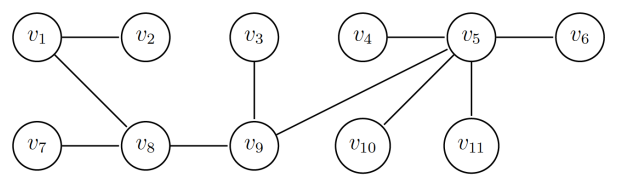
\includegraphics[scale=0.35]{27.png}
\end{figure}

\begin{table}[h!]
    \centering
    \begin{tabular}{|c|c|c||c|c|c||c|c|c|}
    \hline
    $i$ & Вершина & $p_i$ & $i$ & Вершина & $p_i$ & $i$ & Вершина & $p_i$ \\
    \hline
    1 & $v_2$ & 1 & 4 & $v_4$ & 5 & 7 & $v_8$ & 9 \\
    2 & $v_1$ & 8 & 5 & $v_6$ & 5 & 8 & $v_9$ & 5 \\
    3 & $v_3$ & 9 & 6 & $v_7$ & 8 & 9 & $v_{10}$ & 5 \\
    \hline
    \end{tabular}
\end{table}

Получаем следующий код Прюфера: $P=\set{1,8,9,5,5,8,9,5,5}$

В код Прюфера входят только вершины, не являющиеся висячими.
При этом они участвуют в коде $\delta(v)$ -- 1 раз.

\textbf{Алгоритм восстановления дерева:}
\begin{enumerate}[left=0.0em, labelsep=1em, topsep=0.0em, itemsep=0pt, parsep=0.5em]
    \item Записываем код дерева в первой строке. Находим количество вершин
    в дереве (число чисел в коде плюс 2) Во второй строке выписываем вершины,
    которых нет в коде (висячие вершины).
    \item Берём вершину $u$ -- первую вершину в первой строке и вершину $v$ --
    вершину с минимальным номером из второй строки. Записываем ребро $(u, v)$
    и вычёркиваем $u$ и $v$ из соответствующих строк. Если вершины $u$ больше нет
    в первой строке, то записываем её во вторую строку.
    \item Если вершин в первой строке не осталось, то из оставшихся двух
    вершин нижней строки составляем ребро и останавливаем алгоритм, иначе
    переходим к шагу 2.
\end{enumerate}

Пример. Восстановим дерево по коду Прюфера из примера выше.
\begin{multicols}{2}
    \begin{enumerate}[left=0.0em, labelsep=1em, topsep=0.0em, itemsep=0pt, parsep=0.5em]
        \item Записываем код в первой строке, висячие вершины во второй:\\
        \textbf{1},8,9,5,5,8,9,5,5 (n=11)\\
        \textbf{2},3,4,6,7,10,11
        \item Записываем ребро (1,2)\\
        \textbf{8},9,5,5,8,9,5,5\\
        3,4,6,7,10,11,\textbf{1}
        \item Записываем ребро (8,1)\\
        \textbf{9},5,5,8,9,5,5\\
        \textbf{3},4,6,7,10,11
        \item Записываем ребро (9,3)\\
        \textbf{5},5,8,9,5,5\\
        \textbf{4},6,7,10,11
        \item Записываем ребро (5,4)\\
        \textbf{5},8,9,5,5\\
        \textbf{6},7,10,11
        \item Записываем ребро (5,6)\\
        \textbf{8},9,5,5\\
        \textbf{7},10,11
        \item Записываем ребро (8,7)\\
        \textbf{9},5,5\\
        10,11,\textbf{8}
        \item Записываем ребро (9,8)\\
        \textbf{5},5\\
        10,11,\textbf{9}
        \item Записываем ребро (5,9)\\
        \textbf{5}\\
        \textbf{10},11
        \item Записываем ребро (5,10)\\
        11,5
        \item Записываем ребро (5,11)
    \end{enumerate}
\end{multicols}

Получили граф, соответствующий графу, код которого получали в
предыдущем примере.